\section{Discussion}
\normalsize{
TreadWill is an online tool to deliver automated intervention for depressive symptoms. TreadWill assists patients with depressive symptoms in interactively learning the principles of Cognitive Behavioral Therapy (CBT) and engaging in mindfulness exercises. Additionally, it contains a chatbot with empathy and games based on Cognitive Bias Modification (CBM).\cite{Ghosh2021.11.24.21266799}\\
Reading "Cognitive Behavior Therapy, Second Edition - Basics and Beyond-Judith S. Beck Ph.D. Aaron T. Be"\cite{beck2011cognitive} throughout the first few weeks of the project helped me learn more about Cognitive Behavioural Therapy. In the following weeks, I learned more about finite state machines and implemented a few sample FSMs with their state transition diagrams using Python's pytransitions module.\\

During the month of June, I worked on the installation of the Apache HTTP server and obtained understanding of the Angular and Django web app development frameworks. During this time, I also worked with the Apache HTTP server. Ubuntu needed to be installed on the local PC before I could configure Apache HTTP Server. In addition, I had created multiple instances of the application and hosted them on the Apache HTTP server on various ports of the local machine. I had also configured the Apache server in such a way that any device connected to my Local Area Network (LAN) could access the website that was hosted on the IP address of my computer. The front-end is hosted on the Apache server that was previously described, while the back-end, which is built on Django, is housed on the Daphne server.\\

Working on computer networking is primarily intended to address the Cross-Origin Resource Sharing issues impeding the progress of the treadwill project. Cross-Origin Resource Sharing (CORS) is a standard that allows a server to relax the same-origin policy. This is used to explicitly allow some cross-origin requests while rejecting others.\cite{cors-mozilla} In order to fix the issue without the use of any workarounds, I'm also attempting to simulate a CORS scenario on my own PC by developing a web application utilising the Apache and Daphne servers.\\
}
\clearpage

\begin{figure}[h!]
    \centering
    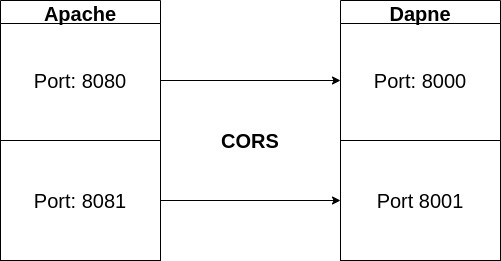
\includegraphics[width=0.7\textwidth,keepaspectratio]{images/workflow-treadwill-Page-2.drawio.png}
    \caption*{CORS in our project}
\end{figure}

\normalsize{
In order to generate the CORS issue, we used multiple instances of the Apache and Daphne servers, each of which was connected to a unique port on the local system.
Consider the following scenario as an illustration: two instances of the application are currently operating on Apache servers that are hosted on ports 8080 and 8081, and two daphne servers are now operating on ports 8000 and 8001. Now that the servers have been setup, the front-end port 8080 is able to interact with the back-end port 8000, while the front-end port 8081 is able to communicate with the back-end port 8001. During this phase of the communication process, the CORS policy is violated, which causes an error in the web browser.\\

We are also actively gathering CBT data for training the Natural Language Processing component of WillBot.
}